%&pdflatex
\documentclass{article}\usepackage[]{graphicx}\usepackage[]{color}
%% maxwidth is the original width if it is less than linewidth
%% otherwise use linewidth (to make sure the graphics do not exceed the margin)
\makeatletter
\def\maxwidth{ %
  \ifdim\Gin@nat@width>\linewidth
    \linewidth
  \else
    \Gin@nat@width
  \fi
}
\makeatother

\definecolor{fgcolor}{rgb}{0.345, 0.345, 0.345}
\newcommand{\hlnum}[1]{\textcolor[rgb]{0.686,0.059,0.569}{#1}}%
\newcommand{\hlstr}[1]{\textcolor[rgb]{0.192,0.494,0.8}{#1}}%
\newcommand{\hlcom}[1]{\textcolor[rgb]{0.678,0.584,0.686}{\textit{#1}}}%
\newcommand{\hlopt}[1]{\textcolor[rgb]{0,0,0}{#1}}%
\newcommand{\hlstd}[1]{\textcolor[rgb]{0.345,0.345,0.345}{#1}}%
\newcommand{\hlkwa}[1]{\textcolor[rgb]{0.161,0.373,0.58}{\textbf{#1}}}%
\newcommand{\hlkwb}[1]{\textcolor[rgb]{0.69,0.353,0.396}{#1}}%
\newcommand{\hlkwc}[1]{\textcolor[rgb]{0.333,0.667,0.333}{#1}}%
\newcommand{\hlkwd}[1]{\textcolor[rgb]{0.737,0.353,0.396}{\textbf{#1}}}%

\usepackage{framed}
\makeatletter
\newenvironment{kframe}{%
 \def\at@end@of@kframe{}%
 \ifinner\ifhmode%
  \def\at@end@of@kframe{\end{minipage}}%
  \begin{minipage}{\columnwidth}%
 \fi\fi%
 \def\FrameCommand##1{\hskip\@totalleftmargin \hskip-\fboxsep
 \colorbox{shadecolor}{##1}\hskip-\fboxsep
     % There is no \\@totalrightmargin, so:
     \hskip-\linewidth \hskip-\@totalleftmargin \hskip\columnwidth}%
 \MakeFramed {\advance\hsize-\width
   \@totalleftmargin\z@ \linewidth\hsize
   \@setminipage}}%
 {\par\unskip\endMakeFramed%
 \at@end@of@kframe}
\makeatother

\definecolor{shadecolor}{rgb}{.97, .97, .97}
\definecolor{messagecolor}{rgb}{0, 0, 0}
\definecolor{warningcolor}{rgb}{1, 0, 1}
\definecolor{errorcolor}{rgb}{1, 0, 0}
\newenvironment{knitrout}{}{} % an empty environment to be redefined in TeX

\usepackage{alltt}
\usepackage{amsmath, amssymb}
\usepackage{geometry}
\geometry{verbose,tmargin=2.5cm,bmargin=2.5cm,lmargin=2.5cm,rmargin=2.5cm}
\setcounter{secnumdepth}{2}
\setcounter{tocdepth}{2}
\usepackage{url}
\usepackage[unicode=false,pdfusetitle,
 bookmarks=true,bookmarksnumbered=true,bookmarksopen=true,bookmarksopenlevel=2,
 breaklinks=false,pdfborder={0 0 1},backref=false,colorlinks=false]
 {hyperref}
\hypersetup{
 pdfstartview={XYZ null null 1}}
\setlength\parindent{0pt}

%\VignetteIndexEntry{An R package for deconvoluting off-target confounded RNAi screens}
%\VignetteDepends{gespeR}
%\VignetteEngine{knitr::knitr}
\IfFileExists{upquote.sty}{\usepackage{upquote}}{}
\begin{document}


\title{Estimating Gene-Specific Phenotpes with \texttt{gespeR}}
\author{Fabian Schmich}

\maketitle
\tableofcontents

\section{The \texttt{gespeR} Model}
This package provides algorithms for deconvoluting off-target confounded phenotypes from RNA interference screens. The packages uses (predicted) siRNA-to-gene target relations in a regularised linear regression model, in order to infer individual gene-specific phenotype (GSP) contributions. The observed siRNA-specific phenotypes (SSPs) for reagent $i = 1,\ldots,n$ as the weighted linear sum of GSPs of all targeted genes $j = 1,\ldots,p$
\begin{align}
Y_i &= x_{i1}\beta_j + \ldots + x_{ip}\beta_p + \epsilon_i,
\end{align}
where $x_{ij}$ represents the strength of knockdown of reagent $i$ on gene $j$, $\beta_j$ corresponds to the GSP of gene $j$ and $\epsilon_i$ is the error term for SSP $i$. The linear reegression model is fit using elastic net regularization:
\begin{align}
\hat{\beta} &= \underset{\beta}{\text{argmin}} \left\{ \sum_{i=1}^n \left( y_i - \sum_{j=1}^p x_{ij}\beta_j \right)^2 + \lambda \sum_{j=1}^p \left(  \alpha\beta_j^2 + \left(1 - \alpha \right) |\beta_j| \right) \right\}.
\end{align}
Here $\lambda$ determines the amount of regualrisation and $\alpha$ is the mixing parameter between the ridge and lasso penalty with $0 \leq \alpha \leq 1$. The elastic net penalty selects variables like the lasso and shrinks together the coefficients of correlated predictors like ridge. This allows for a sparse solution of nonzero GSPs, while retaining simultaneous selection of genes with similar RNAi reagent binding patterns in their respective 3' UTRs. For more information and for citing the \texttt{gespeR} package please use:
\begin{itemize}
\item[]
Schmich F (2015).
\emph{gespeR: Gene-Specific Phenotype EstimatoR}.
R package version 1.1.1, \url{http://www.cbg.ethz.ch/software/gespeR}.

\end{itemize}

\section{Working Example}
In this example, we load first load simulated phenotypic readout and siRNA-to-gene target relations. The toy data consists of four screens (A, B, C, D) of 1,000 siRNAs and a limited gene universe of 1,500 genes. Detailed description of how the data was simulated can be accessed using \texttt{?simData}. First, we load the package:
\begin{knitrout}
\definecolor{shadecolor}{rgb}{0.969, 0.969, 0.969}\color{fgcolor}\begin{kframe}
\begin{alltt}
  \hlkwd{library}\hlstd{(gespeR)}
\end{alltt}
\end{kframe}
\end{knitrout}
Now the phenotypes and target relations can be initialised using the \texttt{Phenotypes} and \texttt{TargetRelations} commands. First, we load the four phenotypes vectors:
\begin{knitrout}
\definecolor{shadecolor}{rgb}{0.969, 0.969, 0.969}\color{fgcolor}\begin{kframe}
\begin{alltt}
  \hlstd{phenos} \hlkwb{<-} \hlkwd{lapply}\hlstd{(LETTERS[}\hlnum{1}\hlopt{:}\hlnum{4}\hlstd{],} \hlkwa{function}\hlstd{(}\hlkwc{x}\hlstd{) \{}
    \hlkwd{sprintf}\hlstd{(}\hlstr{"Phenotypes_screen_%s.txt"}\hlstd{, x)}
  \hlstd{\})}
  \hlstd{phenos} \hlkwb{<-} \hlkwd{lapply}\hlstd{(phenos,} \hlkwa{function}\hlstd{(}\hlkwc{x}\hlstd{) \{}
    \hlkwd{Phenotypes}\hlstd{(}\hlkwd{system.file}\hlstd{(}\hlstr{"extdata"}\hlstd{, x,} \hlkwc{package}\hlstd{=}\hlstr{"gespeR"}\hlstd{),}
      \hlkwc{type} \hlstd{=} \hlstr{"SSP"}\hlstd{,}
      \hlkwc{col.id} \hlstd{=} \hlnum{1}\hlstd{,}
      \hlkwc{col.score} \hlstd{=} \hlnum{2}\hlstd{)}
  \hlstd{\})}
  \hlkwd{show}\hlstd{(phenos[[}\hlnum{1}\hlstd{]])}
\end{alltt}
\begin{verbatim}
## 1000 SSP Phenotypes
## 
## Source: local data frame [1,000 x 2]
## 
##              ID      Scores
## 1  siRNAID_0001 -0.93028719
## 2  siRNAID_0002 -1.12820384
## 3  siRNAID_0003 -1.05265043
## 4  siRNAID_0004  0.80792721
## 5  siRNAID_0005 -1.41533349
## 6  siRNAID_0006  1.64265769
## 7  siRNAID_0007 -0.15733945
## 8  siRNAID_0008  0.74758974
## 9  siRNAID_0009 -0.95904664
## 10 siRNAID_0010 -0.04401824
## ..          ...         ...
\end{verbatim}
\end{kframe}
\end{knitrout}

A visual representation of the phenotypes can be obtained with the \texttt{plot} method:
\begin{knitrout}
\definecolor{shadecolor}{rgb}{0.969, 0.969, 0.969}\color{fgcolor}\begin{kframe}
\begin{alltt}
  \hlkwd{plot}\hlstd{(phenos[[}\hlnum{1}\hlstd{]])}
\end{alltt}


{\ttfamily\noindent\itshape\color{messagecolor}{\#\# stat\_bin: binwidth defaulted to range/30. Use 'binwidth = x' to adjust this.}}\end{kframe}

{\centering 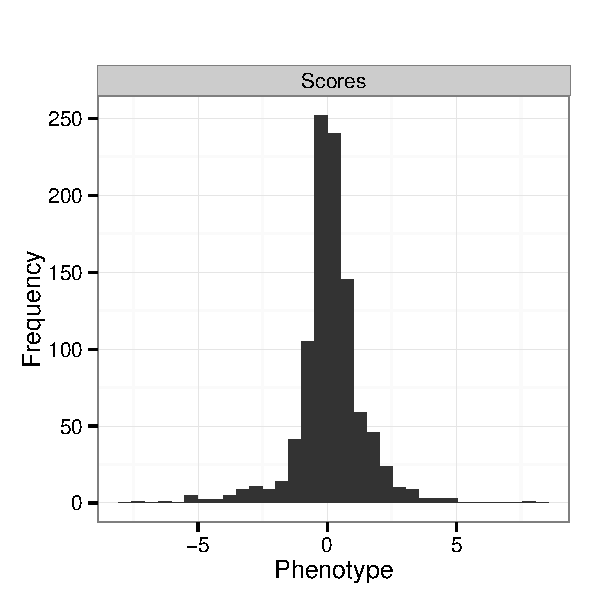
\includegraphics[width=.75\textwidth]{tmp/gespeR-plot_phenotypes-1} 

}



\end{knitrout}

Now, we load the target relations for all four screens using the constructor of the \texttt{TargetRelations} class:
\begin{knitrout}
\definecolor{shadecolor}{rgb}{0.969, 0.969, 0.969}\color{fgcolor}\begin{kframe}
\begin{alltt}
  \hlstd{tr} \hlkwb{<-} \hlkwd{lapply}\hlstd{(LETTERS[}\hlnum{1}\hlopt{:}\hlnum{4}\hlstd{],} \hlkwa{function}\hlstd{(}\hlkwc{x}\hlstd{) \{}
    \hlkwd{sprintf}\hlstd{(}\hlstr{"TR_screen_%s.rds"}\hlstd{, x)}
  \hlstd{\})}
  \hlstd{tr} \hlkwb{<-} \hlkwd{lapply}\hlstd{(tr,} \hlkwa{function}\hlstd{(}\hlkwc{x}\hlstd{) \{}
    \hlkwd{TargetRelations}\hlstd{(}\hlkwd{system.file}\hlstd{(}\hlstr{"extdata"}\hlstd{, x,} \hlkwc{package}\hlstd{=}\hlstr{"gespeR"}\hlstd{))}
  \hlstd{\})}
  \hlkwd{show}\hlstd{(tr[[}\hlnum{2}\hlstd{]])}
\end{alltt}
\begin{verbatim}
## 1000 x 1500 siRNA-to-gene relations.
## 10 x 5 sparse Matrix of class "dgCMatrix"
##               colnames
## rownames       geneID_0001 geneID_0002 geneID_0003 geneID_0004 geneID_0005
##   siRNAID_0001           .   .                   .           .           .
##   siRNAID_0002           .   .                   .           .           .
##   siRNAID_0003           .   0.4385757           .           .           .
##   siRNAID_0004           .   .                   .           .           .
##   siRNAID_0005           .   .                   .           .           .
##   siRNAID_0006           .   .                   .           .           .
##   siRNAID_0007           .   .                   .           .           .
##   siRNAID_0008           .   .                   .           .           .
##   siRNAID_0009           .   .                   .           .           .
##   siRNAID_0010           .   .                   .           .           .
## ...
\end{verbatim}
\end{kframe}
\end{knitrout}

For large data sets, e.g. genome--wide screens, target relations objects can become very big and the user may not want to keep all values in the RAM. For this purpose, we can use the \texttt{unloadValues} method. In this example, we write the values to a temp-file, i.e. not the original source file, which may be required, when we do not want to overwrite exisiting data, after, for instance, subsetting the target relations object.
\begin{knitrout}
\definecolor{shadecolor}{rgb}{0.969, 0.969, 0.969}\color{fgcolor}\begin{kframe}
\begin{alltt}
  \hlcom{# Size of object with loaded values}
  \hlkwd{format}\hlstd{(}\hlkwd{object.size}\hlstd{(tr[[}\hlnum{1}\hlstd{]]),} \hlkwc{units} \hlstd{=} \hlstr{"Kb"}\hlstd{)}
\end{alltt}
\begin{verbatim}
## [1] "678.5 Kb"
\end{verbatim}
\begin{alltt}
  \hlstd{tempfile} \hlkwb{<-} \hlkwd{paste}\hlstd{(}\hlkwd{tempfile}\hlstd{(}\hlkwc{pattern} \hlstd{=} \hlstr{"file"}\hlstd{,} \hlkwc{tmpdir} \hlstd{=} \hlkwd{tempdir}\hlstd{()),} \hlstr{".rds"}\hlstd{,} \hlkwc{sep}\hlstd{=}\hlstr{""}\hlstd{)}
  \hlstd{tr[[}\hlnum{1}\hlstd{]]} \hlkwb{<-} \hlkwd{unloadValues}\hlstd{(tr[[}\hlnum{1}\hlstd{]],} \hlkwc{writeValues} \hlstd{=} \hlnum{TRUE}\hlstd{,} \hlkwc{path} \hlstd{= tempfile)}

  \hlcom{# Size of object after unloading}
  \hlkwd{format}\hlstd{(}\hlkwd{object.size}\hlstd{(tr[[}\hlnum{1}\hlstd{]]),} \hlkwc{units} \hlstd{=} \hlstr{"Kb"}\hlstd{)}
\end{alltt}
\begin{verbatim}
## [1] "159.2 Kb"
\end{verbatim}
\begin{alltt}
  \hlcom{# Reload values}
  \hlstd{tr[[}\hlnum{1}\hlstd{]]} \hlkwb{<-} \hlkwd{loadValues}\hlstd{(tr[[}\hlnum{1}\hlstd{]])}
\end{alltt}
\end{kframe}
\end{knitrout}


In order to obtain deconvoluted gene-specific phenotypes (GSPs), we fit four models on the four separate data sets using cross validation by setting \texttt{mode = "cv"}. We set the elastic net mixing parameter to 0.5 and use only one core in this example:
\begin{knitrout}
\definecolor{shadecolor}{rgb}{0.969, 0.969, 0.969}\color{fgcolor}\begin{kframe}
\begin{alltt}
  \hlstd{res.cv} \hlkwb{<-} \hlkwd{lapply}\hlstd{(}\hlnum{1}\hlopt{:}\hlkwd{length}\hlstd{(phenos),} \hlkwa{function}\hlstd{(}\hlkwc{i}\hlstd{) \{}
    \hlkwd{gespeR}\hlstd{(}\hlkwc{phenotypes} \hlstd{= phenos[[i]],}
          \hlkwc{target.relations} \hlstd{= tr[[i]],}
           \hlkwc{mode} \hlstd{=} \hlstr{"cv"}\hlstd{,}
           \hlkwc{alpha} \hlstd{=} \hlnum{0.5}\hlstd{,}
           \hlkwc{ncores} \hlstd{=} \hlnum{1}\hlstd{)}
  \hlstd{\})}
\end{alltt}
\end{kframe}
\end{knitrout}

The \texttt{ssp} and \texttt{gsp} methods can be used to obtain SSP and GSP scores from a \texttt{gespeR} object:
\begin{knitrout}
\definecolor{shadecolor}{rgb}{0.969, 0.969, 0.969}\color{fgcolor}\begin{kframe}
\begin{alltt}
  \hlkwd{ssp}\hlstd{(res.cv[[}\hlnum{1}\hlstd{]])}
\end{alltt}
\begin{verbatim}
## 1000 SSP Phenotypes
## 
## Source: local data frame [1,000 x 2]
## 
##              ID      Scores
## 1  siRNAID_0001 -0.93028719
## 2  siRNAID_0002 -1.12820384
## 3  siRNAID_0003 -1.05265043
## 4  siRNAID_0004  0.80792721
## 5  siRNAID_0005 -1.41533349
## 6  siRNAID_0006  1.64265769
## 7  siRNAID_0007 -0.15733945
## 8  siRNAID_0008  0.74758974
## 9  siRNAID_0009 -0.95904664
## 10 siRNAID_0010 -0.04401824
## ..          ...         ...
\end{verbatim}
\begin{alltt}
  \hlkwd{gsp}\hlstd{(res.cv[[}\hlnum{1}\hlstd{]])}
\end{alltt}
\begin{verbatim}
## 1500 GSP Phenotypes
## 
## Source: local data frame [1,500 x 2]
## 
##             ID Scores
## 1  geneID_0001     NA
## 2  geneID_0002     NA
## 3  geneID_0003     NA
## 4  geneID_0004     NA
## 5  geneID_0005     NA
## 6  geneID_0006     NA
## 7  geneID_0007     NA
## 8  geneID_0008     NA
## 9  geneID_0009     NA
## 10 geneID_0010     NA
## ..         ...    ...
\end{verbatim}
\begin{alltt}
  \hlkwd{head}\hlstd{(}\hlkwd{scores}\hlstd{(res.cv[[}\hlnum{1}\hlstd{]]))}
\end{alltt}
\begin{verbatim}
## Source: local data frame [6 x 2]
## 
##            ID Scores
## 1 geneID_0001     NA
## 2 geneID_0002     NA
## 3 geneID_0003     NA
## 4 geneID_0004     NA
## 5 geneID_0005     NA
## 6 geneID_0006     NA
\end{verbatim}
\end{kframe}
\end{knitrout}

The fitted models can also be visualised using the \texttt{plot} method:
\begin{knitrout}
\definecolor{shadecolor}{rgb}{0.969, 0.969, 0.969}\color{fgcolor}\begin{kframe}
\begin{alltt}
  \hlkwd{plot}\hlstd{(res.cv[[}\hlnum{1}\hlstd{]])}
\end{alltt}


{\ttfamily\noindent\itshape\color{messagecolor}{\#\# stat\_bin: binwidth defaulted to range/30. Use 'binwidth = x' to adjust this.}}\end{kframe}

{\centering 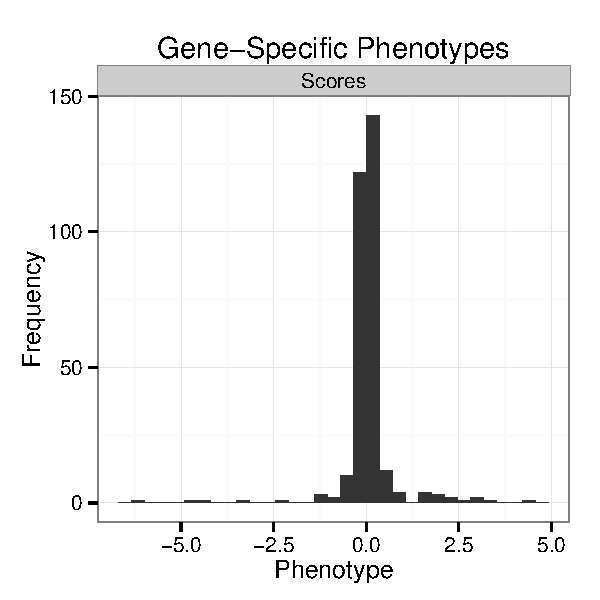
\includegraphics[width=.75\textwidth]{tmp/gespeR-plot_cv-1} 

}



\end{knitrout}


Another way to fit \texttt{gespeR} models is to use stability selection:
\begin{knitrout}
\definecolor{shadecolor}{rgb}{0.969, 0.969, 0.969}\color{fgcolor}\begin{kframe}
\begin{alltt}
  \hlstd{res.stab} \hlkwb{<-} \hlkwd{lapply}\hlstd{(}\hlnum{1}\hlopt{:}\hlkwd{length}\hlstd{(phenos),} \hlkwa{function}\hlstd{(}\hlkwc{i}\hlstd{) \{}
    \hlkwd{gespeR}\hlstd{(}\hlkwc{phenotypes} \hlstd{= phenos[[i]],}
      \hlkwc{target.relations} \hlstd{= tr[[i]],}
      \hlkwc{mode} \hlstd{=} \hlstr{"stability"}\hlstd{,}
      \hlkwc{nbootstrap} \hlstd{=} \hlnum{100}\hlstd{,}
      \hlkwc{fraction} \hlstd{=} \hlnum{0.67}\hlstd{,}
      \hlkwc{threshold} \hlstd{=} \hlnum{0.75}\hlstd{,}
      \hlkwc{EV} \hlstd{=} \hlnum{1}\hlstd{,}
      \hlkwc{weakness} \hlstd{=} \hlnum{0.8}\hlstd{,}
      \hlkwc{ncores} \hlstd{=} \hlnum{1}\hlstd{)}
  \hlstd{\})}
\end{alltt}
\end{kframe}
\end{knitrout}

Again, these models can be visualised using the \texttt{plot} method. This time, the phenotypic scores are plotted against their stability value:
\begin{knitrout}
\definecolor{shadecolor}{rgb}{0.969, 0.969, 0.969}\color{fgcolor}\begin{kframe}
\begin{alltt}
  \hlkwd{plot}\hlstd{(res.stab[[}\hlnum{1}\hlstd{]])}
\end{alltt}
\end{kframe}

{\centering 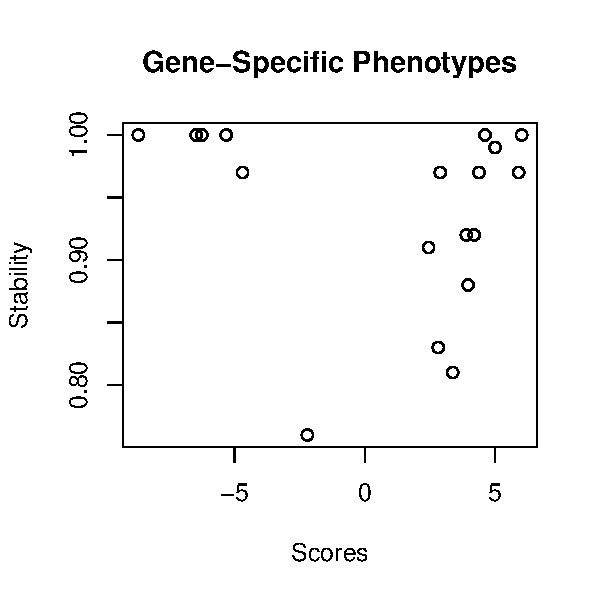
\includegraphics[width=.75\textwidth]{tmp/gespeR-plot_stability-1} 

}



\end{knitrout}

The \texttt{concordance} method can be used to compute the concordance between ranked lists of phenotypes. Here we compute concordance between all pairs of GSPs, as well as between all pairs of SSPs, from all four data sets:
\begin{knitrout}
\definecolor{shadecolor}{rgb}{0.969, 0.969, 0.969}\color{fgcolor}\begin{kframe}
\begin{alltt}
  \hlstd{conc.gsp} \hlkwb{<-} \hlkwd{concordance}\hlstd{(}\hlkwd{lapply}\hlstd{(res.stab, gsp))}
  \hlstd{conc.ssp} \hlkwb{<-} \hlkwd{concordance}\hlstd{(}\hlkwd{lapply}\hlstd{(res.stab, ssp))}
\end{alltt}
\end{kframe}
\end{knitrout}

We can visualise the \texttt{concordance} objects using the \texttt{plot} method:
\begin{knitrout}
\definecolor{shadecolor}{rgb}{0.969, 0.969, 0.969}\color{fgcolor}\begin{kframe}
\begin{alltt}
  \hlkwd{plot}\hlstd{(conc.gsp)} \hlopt{+} \hlkwd{ggtitle}\hlstd{(}\hlstr{"GSPs\textbackslash{}n"}\hlstd{)}
  \hlkwd{plot}\hlstd{(conc.ssp)} \hlopt{+} \hlkwd{ggtitle}\hlstd{(}\hlstr{"SSPs\textbackslash{}n"}\hlstd{)}
\end{alltt}
\end{kframe}

{\centering 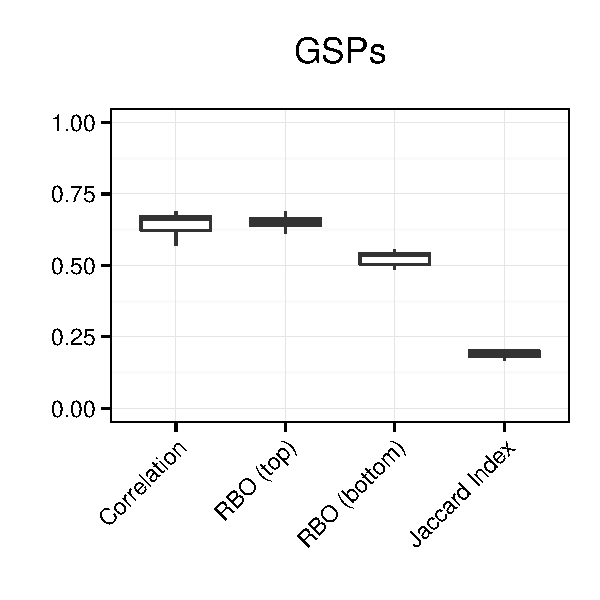
\includegraphics[width=.45\textwidth]{tmp/gespeR-plot_concordance-1} 
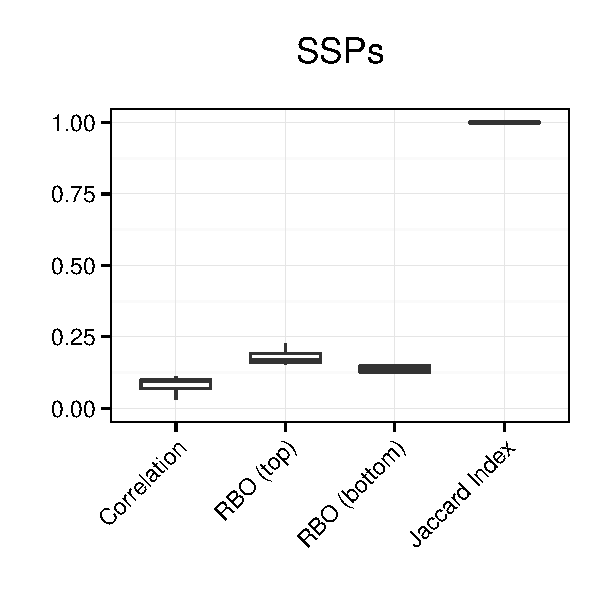
\includegraphics[width=.45\textwidth]{tmp/gespeR-plot_concordance-2} 

}



\end{knitrout}


\section{sessionInfo()}
\begin{itemize}\raggedright
  \item R version 3.2.0 (2015-04-16), \verb|x86_64-apple-darwin13.4.0|
  \item Locale: \verb|en_US.UTF-8/en_US.UTF-8/en_US.UTF-8/C/en_US.UTF-8/en_US.UTF-8|
  \item Base packages: base, datasets, graphics, grDevices,
    methods, stats, utils
  \item Other packages: gespeR~1.1.1, ggplot2~1.0.1, knitr~1.10.5
  \item Loaded via a namespace (and not attached): affy~1.46.1,
    affyio~1.36.0, annotate~1.46.0, AnnotationDbi~1.30.1,
    assertthat~0.1, Biobase~2.28.0, BiocGenerics~0.14.0,
    BiocInstaller~1.18.3, biomaRt~2.24.0, bitops~1.0-6,
    Category~2.34.2, cellHTS2~2.32.0, cluster~2.0.2,
    codetools~0.2-11, colorspace~1.2-6, compiler~3.2.0, DBI~0.3.1,
    DEoptimR~1.0-2, digest~0.6.8, doParallel~1.0.8, dplyr~0.4.2,
    evaluate~0.7, foreach~1.4.2, formatR~1.2, genefilter~1.50.0,
    GenomeInfoDb~1.4.1, glmnet~2.0-2, graph~1.46.0, grid~3.2.0,
    GSEABase~1.30.2, gtable~0.1.2, highr~0.5, IRanges~2.2.4,
    iterators~1.0.7, labeling~0.3, lattice~0.20-31, limma~3.24.10,
    magrittr~1.5, MASS~7.3-41, Matrix~1.2-1, munsell~0.4.2,
    mvtnorm~1.0-2, parallel~3.2.0, pcaPP~1.9-60, plyr~1.8.3,
    prada~1.44.0, preprocessCore~1.30.0, proto~0.3-10, R6~2.0.1,
    RBGL~1.44.0, RColorBrewer~1.1-2, Rcpp~0.11.6, RCurl~1.95-4.6,
    reshape2~1.4.1, robustbase~0.92-4, rrcov~1.3-8, RSQLite~1.0.0,
    S4Vectors~0.6.0, scales~0.2.5, splines~3.2.0, stats4~3.2.0,
    stringi~0.5-2, stringr~1.0.0, survival~2.38-2, tools~3.2.0,
    vsn~3.36.0, XML~3.98-1.2, xtable~1.7-4, zlibbioc~1.14.0
\end{itemize}


\end{document}
